\chapter{RNA編集サイトの検出手法の精度比較}
\label{bench}
\section{研究背景}
RNA-seqデータを用いたRNA編集サイトの検出は、これまでにヒト、マウス、ショウジョウバエを主な対象生物種として情報学的な手法が多数、開発されてきた。RNA編集サイトはゲノムと転写物の一塩基のミスマッチとして検出されるが、シーケンシングやマッピングに起因した擬陽性を多く含む。そのため、ADAR由来のRNA編集サイトと擬陽性とを高精度に分離する検出手法がこれまでに考案されてきた。
\par
ところが、論文ごとに解析対象となる生物種や組織、セルライン、シーケンシング手法などに相違が見られ、各々の手法の検出精度の評価・比較は困難な状況にある。また多くの研究はこれまでに同定された既知の編集サイトとの一致 (共通項)を確認しているに過ぎず、検出結果に含まれる擬陽性の影響を適切に評価するには至っていない。RNA編集サイトを高精度に検出する手法を開発するにあたっては、既知の結果との一致と同時に、検出結果に含まれるノイズとその割合を評価する必要があると考えられる。
\par
バイオインフォマティクスの分野においては、タンパク質の立体構造予測コンテスト CASP (Critical Accesment of protein Structure Prediction)に代表されるように、その分野で開発されたアルゴリズムや手法は、予測精度や計算時間といった複数の指標により性能評価 (Benchmarking test)が実施され、手法の標準化が行われてきた経緯を持つ。本研究もこういった文脈に位置づけることができる。
\par
異なる検出手法についての精度評価は、生物種やサンプル毎に適したフィルタリング手法とそのパラメータを明らかにすることが目的である。序論で前述したとおり、RNA編集サイトの高精度な検出には、様々なフィルタリング手法を複合的に組み合わせることによって擬陽性の排除が行われており、手法ごとにゲノムへのマッピングにおける許容ミスマッチ数、最小のリードカバレッジなど、擬陽性の排除に使用されたフィルタリング手法は異なる。検出手法の性能評価により、高精度な検出手法が明らかとなると、他の手法との差を高精度な検出に寄与するパラメータの候補として抽出することが可能である。このような知見は、汎用性のある新たなRNA編集サイトの検出手法の開発に貢献できると考えられる。
\par
本研究は、ヒト・マウス・ショウジョウバエのRNA-seqデータを用いた既存のRNA編集サイトの検出手法に関する性能評価を行い、高精度な検出に寄与するパラメータの探索を行ったものである。性能評価には再現率および適合率といった指標を導入し、各手法の検出精度について定量的な比較を行った。結果、生物種ごとに検出手法の精度を明らかにした。この結果を受け、シーケンシング手法などの実験デザインおよび検出手法が検出精度にどのように寄与しているのかについて議論する。

\section{対象と手法}
\subsection{性能評価に用いた指標}
これまでに開発されてきたRNA編集サイトの検出手法を統一的な指標によって性能評価を行うため、適合率 (Precision)・再現率 (Recall)・F値 (F-measure)と呼ばれる3つの指標を導入した。この3つの指標は情報工学において検索精度の測定において用いられており、情報検索の結果に対して検索ノイズと検索漏れという2つの側面からアルゴリズムの性能を測定するものである。
\par
以下にぞれぞれの指標とその計算方法について示す。この3つの指標は、算出される値が高いほど高精度であることを表す。以下で説明する際の検出サイトは、各手法により検出された全A-to-I編集サイトを指し、正解サイトは過去に報告された既知の全編集サイトを表す。

\subsubsection{適合率 (Precision)}
適合率は、式\ref{eq:precision}に定義される。検出サイトと真のeditingサイトの積集合に対する検出サイトの割合として計算される。適合率は検出サイトに正解が含まれる割合を意味しており、検出サイトの中に正解サイトとの一致が濃縮されることで高い適合率が達成される。
\begin{eqnarray}
	Precision = \frac{TP}{TP + FP} = \frac{CandidateSites \cap TrueEditingSites}{CandidateSites}
	\label{eq:precision}
\end{eqnarray}

\subsubsection{再現率 (Recall)}
再現率は、式\ref{eq:recall}に定義され、正解セットに対して検出サイトが正解した割合を示す。ゲノム中における多くの箇所をedititingサイトとして検出することで原理的に再現率は1に近づくが、一方で擬陽性が増大するため適合率は0に近づく。このように、両者はトレードオフの関係にあることから、正確なRNA編集サイトの検出には、再現率の向上よりも適合率を増加させる手法やパラメータを見出すことが重要である。
\begin{eqnarray}
	Recall = \frac{TP}{TP+FN}
	= \frac{CandidateSites \cap TrueEditingSites}{TrueEditingSites}
	\label{eq:recall}
\end{eqnarray}

\subsubsection{F値 (F-measure)}
F値は、適合率および再現率の調和平均として式\ref{eq:f_measure}のように定義される。F値の導入により、再現率と適合率の2つの評価基準を一元的に取り扱うことが可能となる。
\begin{eqnarray}
	Fmeasure = 2 \times \left( \frac{precision \times recall}{precision + recall} \right)
	\label{eq:f_measure}
\end{eqnarray}

\subsection{正解セットの構築}
検出精度を評価するためには、真のRNA編集の集合を定義した正解セットの構築が必須となる。そこで、これまでの研究によって報告されたA-to-I編集サイトを収集したDARNED (Database of RNA editing site, \url{http://darned.ucc.ie/})と呼ばれるデータベースに登録されている全データをヒト・マウス・ショウジョウバエの3種ごとに取得し、正解セットを構築した。DARNEDは、実験的な手法により同定されたA-to-I編集サイトの他に、情報学的な手法により同定されたサイトの双方を含み、文献と紐付けられた編集サイトに関するメタデータと共に公開している。表\ref{tab:darned}に、生物種ごとに収集した正解セットの総数をまとめた。尚、精度評価の実施にあたり、取得した全てのサイトを正解セットとして扱い、同定手法の如何については区別しなかった。

\begin{longtable}{cccc}
	\vspace{-0.5cm}
	\label{tab:darned}\\
	\caption{DARNEDより収集したA-to-I編集サイトの内訳}\\
	\cline{1-4}
	\textbf{Species} & \textbf{Reference genome version} & \textbf{Studies} & \textbf{Answer sites} \\
	\cline{1-4}
	\textit{H. sapiens} & hg19 & 20 & 333,216 \\
	\textit{H. sapiens} & hg18 & 22 & 259,705 \\
	\textit{M. musclus} & mm10 & 4 & 8,341 \\
	\textit{M. musclus} & mm9  & 4 & 8,352 \\
	\textit{D. melanogaster} & dm3 & 3 & 1,969 \\
	\cline{1-4}
	\vspace{-0.8cm}
\end{longtable}
\begin{flushleft}
	\small{DARNEDにより取得した3種それぞれの正解セットの情報示す。3種それぞれに対応するゲノムのバージョン、正解セットの検出に関わる先行研究の数、収集した正解セットの総数をそれぞれ示す。}
\end{flushleft}

\subsection{性能評価に用いた検出手法}
RNA編集サイトの検出精度に関する性能評価を実施するにあたり、(i) RNA-seqデータを用いた検出手法であること、(ii) シーケンスデータがSequence Read Archive (\url{http://www.ncbi.nlm.nih.gov/sra/})において公開されていること、(iii) 同定されたRNA編集サイトの全リストが取得可能であることを評価の条件とし、ヒト・マウス・ショウジョウバエの3種類からそれぞれ評価する先行研究を選出した。表\ref{tab:methods}にその一覧を示した。一覧では、便宜的に先行研究ごとに分類しているが、先行研究によっては異なる組織やセルラインに多数の解析を行っている場合があるため、この場合に関してはサンプルごとに性能比較を行うようにした。これにより同一手法における組織やセルライン毎での精度の違いを明らかにすることができると考えられた。
\begin{longtable}{cccc}
	\vspace{-0.5cm}
	\label{tab:methods}\\
	\caption{性能評価に用いた検出手法のリスト}\\
	\cline{1-3}
	\bf{Study} & \textbf{Samples (tissue/cell line)} & \textbf{Identified sites} \\
	\bi{H. sapiens} \\
	\cline{1-3}
	%\endhead
	Ramaswami, \textit{et al.,} 2012 & GM12878 (lymphoblastoid cell line) & 74,166 \\
	Ramaswami, \textit{et al.,} 2013 & Lymphocyte cell line & 230,402 \\
	Peng, \textit{et al.,} 2012 & Lymphoblastoid cell line in Han Chinese individual & 22,696 \\
	Park, \textit{et al.,} 2013 & 14 human cell lines (ENCODE project) & 13,821 \\
	Zhu, \textit{et al.,} 2013 & 16 human tissues, 2 cell lines (Illumina BodyMap 2.0) & 2,246 \\
	Bahn, \textit{et al.,} 2012 & U87MG (glioblastoma cell line) & 12,791 \\
	\bi{M. musculs} \\
	\cline{1-3}
	Gu, \textit{et al.,} 2012 & White adipose, Femurs, liver & 244 \\
	Dillman, \textit{et al.,} 2013 & Cerebral cortex, 4 embryonic mice & 177 \\
	Lagarrigue, \textit{et al.,} 2013 & Liver, Adipose & 363 \\
	\bi{D. melanogaster} \\
	\cline{1-3}
	Rodriguez, \textit{et al.,} 2012 & Fly head & 1,351 \\
	Graveley, \textit{et al.,} 2011  & Fly head & 973 \\
	Ramaswami, \textit{et al.,} 2013 & Fly head & 850 \\
	\cline{1-3}
	\vspace{-0.8cm}
\end{longtable}
\begin{flushleft}
	\small{本研究において精度評価の対象となった先行研究の検出手法を生物種ごとに分類して示した。先行研究が用いたセルラインや組織と最終的なA-to-I編集サイトの総数を表記した。異なるセルラインや組織の結果を統合的に解析している場合は、サンプル欄に複数を列挙した。}
\end{flushleft}
\newpage

\section{検出性能の比較結果}
\subsection{生物種毎のごとの精度比較}
\subsubsection{ヒト}
ヒトについては、6つの先行研究について合計27サンプルを用いた性能評価を行った。再現率、適合率による各手法の検出精度を図\ref{fig:human}に示す。対象とした検出手法の全体としての精度の傾向は、どの手法も共通して0.2以下の低い再現率を示し、中でも最も高い再現率は、Alu領域から検出されたサンプルを用いたRamaswami, \textit{et al.,} 2012の0.15だった。適合率については、手法とサンプルによって大きく分散することが示された。適合率に関してはRamaswami \textit{et al.,} 2013が再現率0.98を示し、最も高い手法であることがことが示された (図\ref{fig:human_cr})。ENCODEプロジェクトにおいて、用いられた手法はどのセルラインに対しても共通して低い再現率と適合率を示す傾向が観察された。中でも、セルラインGM12892における再現率が0.13と最も高く、適合率については、0.0005程度とどの手法も極端に低かった。そのため、F値はどのセルラインについても呼応して低い傾向が見られた。F値は、再現率の最も高かったRamaswami, \textit{et el., }2012が0.25であり、最も高いF値を示す手法であることが分かった。
\par
再現率と適合率を用いた性能評価を行ったところ、検出手法ごとに再現率、特に適合率が大きく分散する傾向が観察された。この原因を探るため、再現率および適合率が検出された編集サイト数との関係性についての解析を行った結果を図\ref{fig:human_data}に示す。その結果、高い再現率を示す手法は、検出した編集サイトの総数も60,000サイト以上と相対的に多い傾向が見られた。適合率については、二つのパタンが観察された。適合率が0.3以下のグループでは、適合率の上昇と検出された編集サイト数には、相関は見られず、10,000箇所以上を検出したRamaswami, \textit{el al., }2013の脳のサンプルに対して、1000箇所程度を同定したHSMM、GM12891、GM12892セルラインの方が高い再現率を示した。また、再現率が0.5以上については、この傾向が顕著に見られ、検出サイトの増加と精度の上昇の間に関係性は見られなかった。
\begin{figure}[!h]
	\begin{minipage}{1\textwidth}
	    \centering
		\subfigure[ヒトにおける検出精度の評価結果]{\includegraphics[width=0.8 \hsize]{bench_human.pdf}
		\label{fig:human_cr}}
		\subfigure[検出精度と検出された編集サイト数の関連性]{\includegraphics[width=0.8 \hsize]{Human_correlation.pdf}\label{fig:human_data}}
		\vspace*{4mm}
		\caption{ヒトを対象とした手法の性能評価}
		\label{fig:human}
	\end{minipage}\hfill
	%\vspace*{-5mm}
	\begin{flushleft}
		\small{\textbf{\subref{fig:human_cr}}横軸に適合率、縦軸に再現率をそれぞれ示した。図中の色分けは、手法あるいはセルラインや組織ごとに変えて表した。\textbf{\subref{fig:human_data}}ヒトを対象とした手法について、縦軸にそれぞれの手法によって検出されたA-to-I編集サイト数を示し、横軸に適合率および再現率を図示した。検出精度の指標はそれぞれ黒丸は適合率、黒三角は再現率に対応する。また、青線は適合率および再現率と候補サイト数の単回帰直線を示した。}
	\end{flushleft}
\end{figure}

\subsubsection{マウス}
マウスを対象とした検出手法の性能評価の結果を図\ref{fig:mouse}に示した。再現率は、用いた3つの手法は、最大でもGu \textit{et al., 2012}の0.03が最大であり、極端に低い値を示した。適合率は、Gu \textit{et al., 2012}が最も高い0.99を示し、続いてDillman \textit{et all., 2013}が0.75であることが示された (図\ref{fig:mouse_pr})。図\ref{fig:mouse_data}は、ヒトの解析と同様に検出精度と検出した編集サイト数の関係性をプロットした結果であるが、再現率は検出編集サイト数と3つ全ての手法において正の相関が見られた。対して、適合率は、Lagarrigue, \textit{et al., }2013の手法を除くと、正に相関する傾向が観察された。他の手法とサンプルの3つに関しては、検出数と適合率は強く相関することが示された。
\begin{figure}[!h]
	\begin{center}
		\subfigure[マウスのデータを用いた検出手法の精度評価]{\includegraphics[width=0.5 \hsize]{bench_mouse.pdf}\label{fig:mouse_pr}}
		\subfigure[検出精度と編集サイト数との関連性]{\includegraphics[width=0.49 \hsize]{Mouse_correlation.pdf}\label{fig:mouse_data}}
		\vspace*{4mm}
		\caption{マウスのデータを用いた検出手法の精度評価}
		\label{fig:mouse}
	\end{center}
	\vspace*{-7mm}
	\begin{flushleft}
		\small{\textbf{\subref{fig:mouse_pr}}マウスにおける検出精度の結果を示す。\textbf{\subref{fig:mouse_data}}候補となったA-to-I編集サイト数と検出精度との関係性を示す。青線は、候補サイト数と検出精度の回帰直線を示す。}
	\end{flushleft}
\end{figure}

\subsubsection{ショウジョウバエ}
ショウジョウバエを対象とした検出手法の精度比較の結果を図\ref{fig:dmel}に示す。最大の適合率を示した手法はRodriguez \textit{et al., }2012の0.49であった。また、再現率に関しては、Graveley, \textit{et al., }2011 (modENCODEの手法)が最大を示した。図\ref{fig:fly_data}に示したように、候補となるeditingサイトを多く検出した手法ほど、再現率と適合率が向上するという傾向が確認された。
また、Ramaswami \it{et al}\rm{}., 2013において用いられた検出手法は、再現率ならびに適合率はどちらも他2つの手法に対して低い精度であることが示された。また、Ramaswami \it{et al}\rm{}., 2013において用いられた検出手法は、再現率ならびに適合率はどちらも他2つの手法に対して低い精度であることが示された。また、Ramaswami \it{et al}\rm{}., 2013において用いられた検出手法は、再現率ならびに適合率はどちらも他2つの手法に対して低い精度であることが示された。また、
\begin{figure}[!h]
	\begin{center}
		\subfigure[ショウジョウバエにおける検出手法の精度評価]{\includegraphics[width=0.49 \hsize]{bench_fly.pdf}\label{fig:fly_pr}}
		\subfigure[検出精度と編集サイト数との関係]{\includegraphics[width=0.49 \hsize]{dmel_correlation.pdf}
		\label{fig:fly_data}}
		\vspace*{4mm}
		\caption{ショウジョウバエのデータを用いた検出手法の精度評価}
		\label{fig:dmel}
	\end{center}
	\vspace*{-7mm}
	\begin{flushleft}
		\small{\textbf{\subref{fig:fly_pr}}ショウジョウバエにおける検出精度の結果を示す。\textbf{\subref{fig:fly_data}}候補となったA-to-I編集サイト数と検出精度との関係性を示す。青線は、候補サイト数と検出精度の回帰直線を示す。}
	\end{flushleft}
\end{figure}

\subsection{検出手法の詳細とパラメータ}
図\ref{fig:f_measure}では、今回の精度検証に用いた全手法のF値を示した。

\begin{figure}[!h]
	\begin{center}
		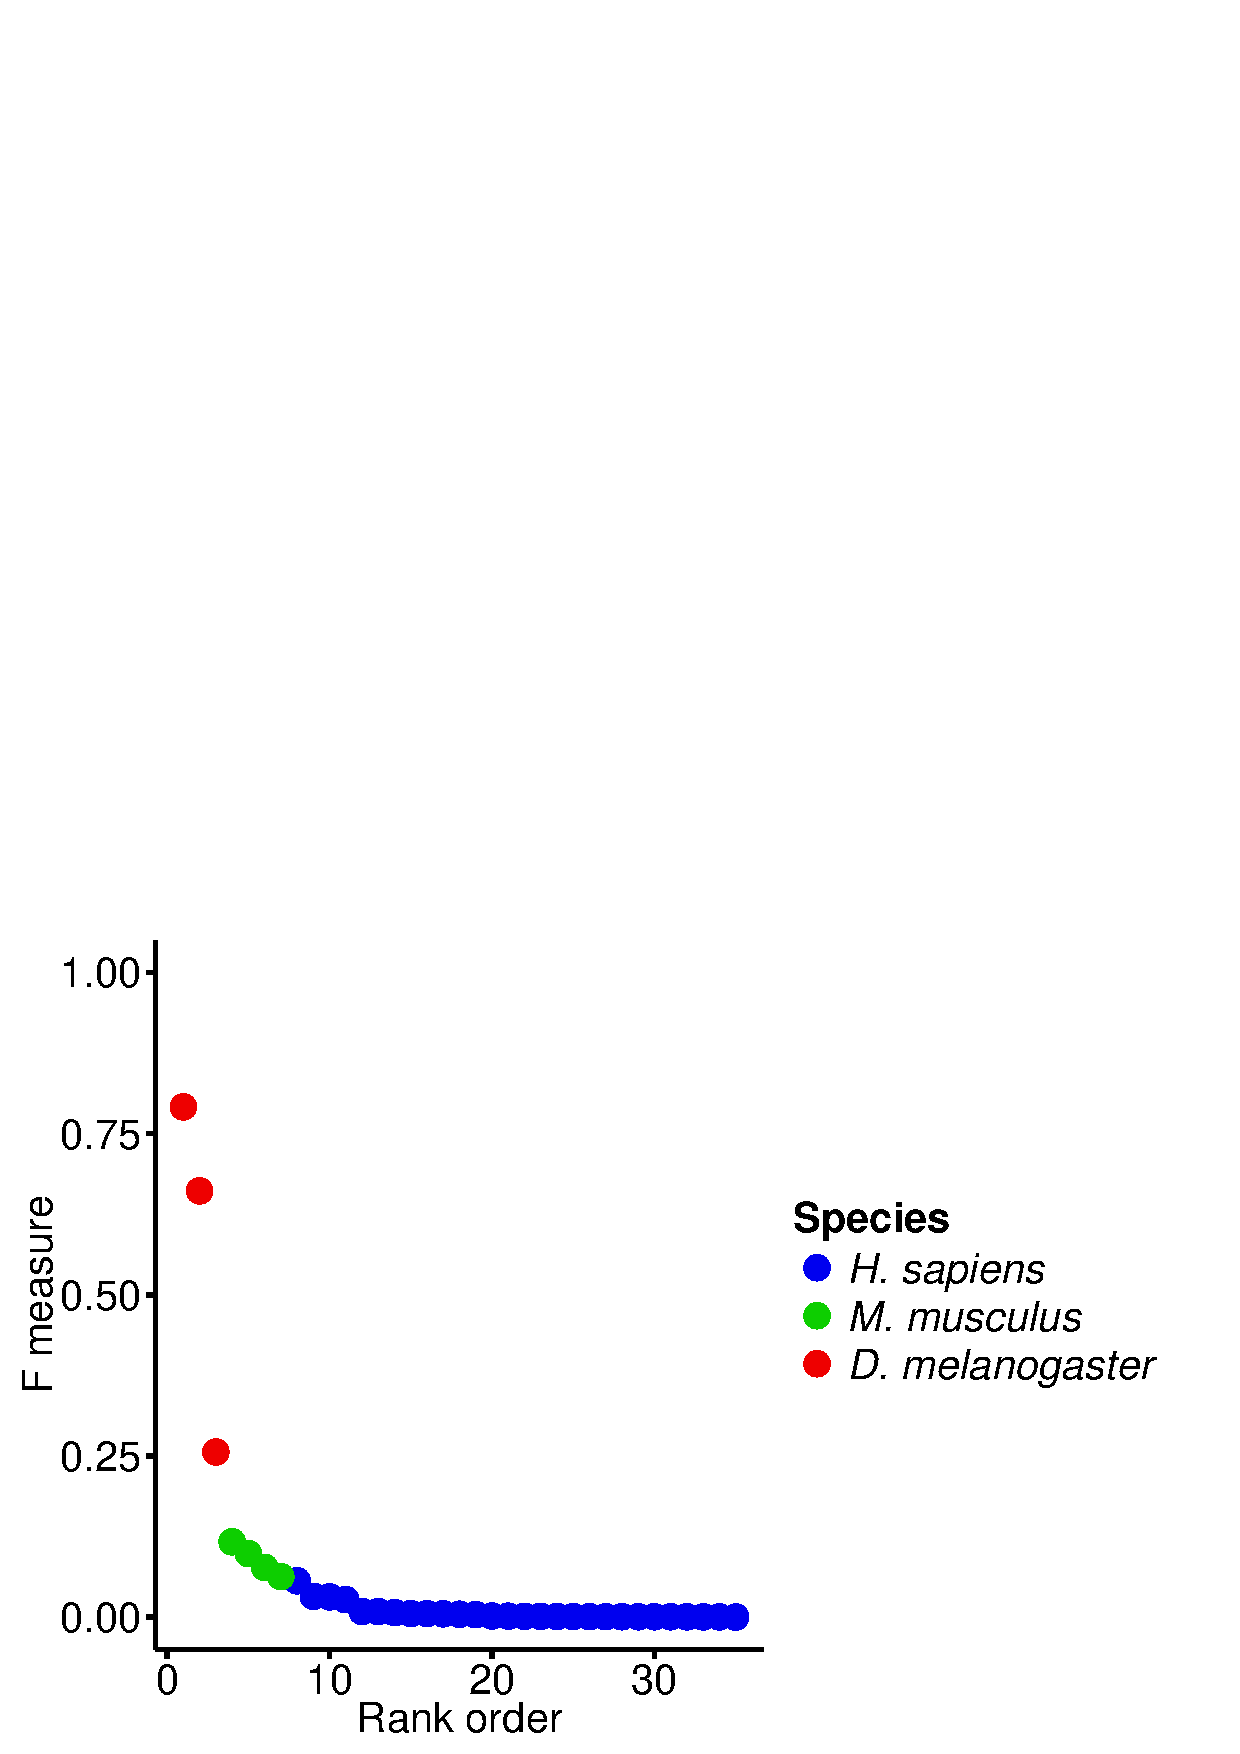
\includegraphics[width=0.7 \hsize]{f_rank_order.pdf}
	\end{center}
	\caption{検出手法ごとのF値の分布}
	\begin{flushleft}
		\small{赤はヒト、青はマウス、緑はショウジョウバエを対象とした手法のF値をそれぞれ示す。}
	\end{flushleft}
	\label{fig:f_measure}
\end{figure}

\begin{landscape}
	\begin{figure}[!h]
		\centering
		\includegraphics[width=0.9 \hsize]{methods_table.pdf}
		\caption{性能評価に用いた検出手法において使用されたフィルタリング手法とそのパラメータ}
		\begin{flushleft}
			\small{赤はヒト、青はマウス、緑はショウジョウバエを対象とした手法をそれぞれ示す。濃くハイライトされた手法は、各生物種において最も精度の高い手法を示す。}
		\end{flushleft}
		\label{Fig:*****}
	\end{figure}
\end{landscape}

\section{議論}
本研究は、情報検索の分野で用いられてきた適合率・再現率およびF値と呼ばれる精度評価の指標を導入し、RNA編集サイトの検出手法の精度を定量化し、異なる複数の手法の直接的な比較を可能にした。先行研究においては、T-to-GやC-to-Aなど全塩基置換の個数を集計し、全体の分布においてA-to-Gへの置換が濃縮されたピークとして見られること、またはDARNEDのデータを使い、既知の報告例との一致の割合を示すことにより、検出手法の妥当性を示してきた。従って検出手法ごとに異なったデータや方法で検出精度の妥当性を評価しており、検出手法を比較することは困難であった。
\par
ヒトを対象にした手法の性能評価によると、どの手法も平均的に低い再現率を示す傾向が見られたが、これはDARNEDから収集した正解セットが330,000箇所以上と検出された編集サイトを数倍上回る母数であったことが原因だと考えられる。この影響を受けて、ヒトのRNA-seqデータに用いられた手法は総じて、低い再現率を示したと考えられる。ENCODEプロジェクトによる解析も低い再現率を示しているが、この原因も同様に検出された編集サイトの総数が正解セットに対して少ないことが原因だと考えられる。ENCODEプロジェクトにおいては、多くのセルラインを用いた解析が行われたが、最終的な検出サイトは1,000から2,000サイト程度であり、これは他の手法による検出された編集サイトの1/10程度である。この傾向を裏付ける結果として、再現率は検出サイト数の増加に対して比例的に上昇する、という傾向が見られている (図\ref{fig:human_data})。再現率の計算上、候補数が増加すると再現率もまた高くなるからである。対して、適合率にはこのような線形的な関係が見られないのは、検出サイト数は増加する分、擬陽性の割合も同時に高くなるため、再現率とは異なる傾向が見られたのだと考えられる。
\par
ヒトのRNA-seqデータを用いた解析では、Ramaswami, \textit{et el., }2012が最も高い精度を持った手法であることが明らかとなった。この手法において精度の高い検出には、実験段階では、Strand-specificシーケンシングの他に\textit{Adar}の変異体を同時にシーケンシングしている点である。また、データ解析においては、ショートリードをゲノムにかぎらず、遺伝子モデルへもマッピングしている点である。このようなリードのマッピング戦略は、スプライスサイト周辺に集中して見られるミスマッチの減少に寄与していると考えられる。また、他の手法に対して、Base call qualityやMapping qualityのしきい値が厳格である他、ホモポリマー領域のフィルタリングを行っている。ホモポリマーは、シーケンサーによる配列決定に誤読が誘発されやすい繰り返し領域である。このような実験デザインおよびフィルタリング手法により、Ramaswami, \textit{et al., }2012は高精度化を達成していると考えられた。
\par
マウスのRNA-seqデータを用いた検出手法は、共通して再現率が極端に低い傾向が示された。この低い再現率の原因は、マウスを用いた検出手法は正解セットに対して、検出した編集サイトが少ない点が考えられる。10,000サイトからなる正解セットに対して、既知のサイトと完全一致 (適合率1.0)した場合にも、再現率は最大でも0.1にとどまるからである。適合率に関しては、少ない母数に正解セットとの一致が濃縮された結果、Gu \textit{et al., }2012やDallman \textit{et al., }2013では高い適合率を示した。
\par
ショウジョウバエにおける検出手法の精度比較を行った結果、再現率に関しては非常に高い結果を示した。
これは正解セットおよび検出手法のどちらもが、ショウジョウバエの頭部から抽出されたRNAであり、組織の同一性が高い再現率に寄与している可能性が考えられる。適合率について議論する。最もF値の高かったRodriguez \textit{et al., }2012は、\textit{Adar}の変異体を用いている。サンプル毎に2つの生物学的レプリケートを使っている。このような実験デザインは、高精度な検出には必要となると考えられる。
\par
本研究は、超並列シーケンサーを用いたRNA編集サイトの検出手法の精度比較を初めて実施した結果、ヒト、マウス、ショウジョウバエにおける複数の検出手法の持つ検出精度を明らかにした。こういった方法は、新たなシーケンシングデータの情報解析にとどまらず、新規の検出手法の開発にも貢献できると考えられる。
\par
今後、より正確な性能評価には、全ての手法において同一のRNA-seqデータを使って再解析する必要があると考えている。本解析では、入力となるRNA-seqデータと手法の双方が先行研究ごとに異なり、純粋に手法のみの比較が行えていない可能性が示唆される。そこで、解析対象となったRNA-seqデータと検出手法の影響を明確に分離し、RNA-seqデータを比較する全ての手法で同一にした上で、性能評価を行う必要があるだろう。そのためには、ENCODEプロジェクトなどの豊富なデータを用いて、純粋な手法の比較を行うことが望まれる。加えて、計算方法が正解セットのサイズに依存的であるため、多数のサイトを検出する手法は高い再現率を示しやすく、これは結果的にF値の上昇に直結する。検出サイト数に応じて正解セットをランダムサンプリングするなどの正解セットの適切な正規化も有効となるとかんがえられる。


